\documentclass[english,,man]{apa6}
\usepackage{lmodern}
\usepackage{amssymb,amsmath}
\usepackage{ifxetex,ifluatex}
\usepackage{fixltx2e} % provides \textsubscript
\ifnum 0\ifxetex 1\fi\ifluatex 1\fi=0 % if pdftex
  \usepackage[T1]{fontenc}
  \usepackage[utf8]{inputenc}
\else % if luatex or xelatex
  \ifxetex
    \usepackage{mathspec}
  \else
    \usepackage{fontspec}
  \fi
  \defaultfontfeatures{Ligatures=TeX,Scale=MatchLowercase}
\fi
% use upquote if available, for straight quotes in verbatim environments
\IfFileExists{upquote.sty}{\usepackage{upquote}}{}
% use microtype if available
\IfFileExists{microtype.sty}{%
\usepackage{microtype}
\UseMicrotypeSet[protrusion]{basicmath} % disable protrusion for tt fonts
}{}
\usepackage{hyperref}
\hypersetup{unicode=true,
            pdftitle={Do Items Order? The Psychology in IRT Models},
            pdfauthor={Julia M. Haaf, Edgar C. Merkle, \& Jeffrey N. Rouder},
            pdfkeywords={Item ordering, Item response theory, Cognitive psychometrics},
            pdfborder={0 0 0},
            breaklinks=true}
\urlstyle{same}  % don't use monospace font for urls
\ifnum 0\ifxetex 1\fi\ifluatex 1\fi=0 % if pdftex
  \usepackage[shorthands=off,main=english]{babel}
\else
  \usepackage{polyglossia}
  \setmainlanguage[]{english}
\fi
\usepackage{graphicx,grffile}
\makeatletter
\def\maxwidth{\ifdim\Gin@nat@width>\linewidth\linewidth\else\Gin@nat@width\fi}
\def\maxheight{\ifdim\Gin@nat@height>\textheight\textheight\else\Gin@nat@height\fi}
\makeatother
% Scale images if necessary, so that they will not overflow the page
% margins by default, and it is still possible to overwrite the defaults
% using explicit options in \includegraphics[width, height, ...]{}
\setkeys{Gin}{width=\maxwidth,height=\maxheight,keepaspectratio}
\IfFileExists{parskip.sty}{%
\usepackage{parskip}
}{% else
\setlength{\parindent}{0pt}
\setlength{\parskip}{6pt plus 2pt minus 1pt}
}
\setlength{\emergencystretch}{3em}  % prevent overfull lines
\providecommand{\tightlist}{%
  \setlength{\itemsep}{0pt}\setlength{\parskip}{0pt}}
\setcounter{secnumdepth}{0}
% Redefines (sub)paragraphs to behave more like sections
\ifx\paragraph\undefined\else
\let\oldparagraph\paragraph
\renewcommand{\paragraph}[1]{\oldparagraph{#1}\mbox{}}
\fi
\ifx\subparagraph\undefined\else
\let\oldsubparagraph\subparagraph
\renewcommand{\subparagraph}[1]{\oldsubparagraph{#1}\mbox{}}
\fi

%%% Use protect on footnotes to avoid problems with footnotes in titles
\let\rmarkdownfootnote\footnote%
\def\footnote{\protect\rmarkdownfootnote}


  \title{Do Items Order? The Psychology in IRT Models}
    \author{Julia M. Haaf\textsuperscript{1}, Edgar C. Merkle\textsuperscript{2}, \& Jeffrey N. Rouder\textsuperscript{3}}
    \date{}
  
\shorttitle{Do Items Order?}
\affiliation{
\vspace{0.5cm}
\textsuperscript{1} University of Amsterdam\\\textsuperscript{2} University of Missouri\\\textsuperscript{3} University of California, Irvine}
\keywords{Item ordering, Item response theory, Cognitive psychometrics}
\usepackage{csquotes}
\usepackage{upgreek}
\captionsetup{font=singlespacing,justification=justified}

\usepackage{longtable}
\usepackage{lscape}
\usepackage{multirow}
\usepackage{tabularx}
\usepackage[flushleft]{threeparttable}
\usepackage{threeparttablex}

\newenvironment{lltable}{\begin{landscape}\begin{center}\begin{ThreePartTable}}{\end{ThreePartTable}\end{center}\end{landscape}}

\makeatletter
\newcommand\LastLTentrywidth{1em}
\newlength\longtablewidth
\setlength{\longtablewidth}{1in}
\newcommand{\getlongtablewidth}{\begingroup \ifcsname LT@\roman{LT@tables}\endcsname \global\longtablewidth=0pt \renewcommand{\LT@entry}[2]{\global\advance\longtablewidth by ##2\relax\gdef\LastLTentrywidth{##2}}\@nameuse{LT@\roman{LT@tables}} \fi \endgroup}


\DeclareDelayedFloatFlavor{ThreePartTable}{table}
\DeclareDelayedFloatFlavor{lltable}{table}
\DeclareDelayedFloatFlavor*{longtable}{table}
\makeatletter
\renewcommand{\efloat@iwrite}[1]{\immediate\expandafter\protected@write\csname efloat@post#1\endcsname{}}
\makeatother
\usepackage{bm}
\usepackage{amsmath}
\usepackage{setspace}
\usepackage{pcl}
\usepackage{marginnote}
\newcommand{\readme}[1]{\emph{\marginnote{Ed} (#1)}}

\authornote{This paper was written using knitr and R Markdown. Using these tools, the text and the code for analysis may be included in a single document. The document for this paper, with all text and code, may be found at \url{https://github.com/PerceptionAndCognitionLab/irt-2pe}.

Correspondence concerning this article should be addressed to Julia M. Haaf, Department of Psychology, PO Box 15906, 1001 NK Amsterdam, The Netherlands.. E-mail: \href{mailto:jhaaf@mail.missouri.edu}{\nolinkurl{jhaaf@mail.missouri.edu}}}

\abstract{
Invariant item ordering refers to the statement that if one item is harder than another for one person, then it is harder for all people. Whether item ordering holds is a psychological statement because it describes how people may qualitatively vary. Yet, modern item response theory (IRT) makes an \emph{a priori} commitment to item ordering. The Rasch model, for example, posits that items must order. Conversely, the 2PL model posits that items never order. Needed is an IRT model where item ordering or its violation is a function of the data rather than an \emph{a priori} commitment. We develop two-parameter shift-scale models for this purpose, and find that the two-parameter uniform offers many advantages. We show how item ordering may be assessed using Bayes factor model comparison, and discuss computational issues with shift-scale IRT models.


}

\begin{document}
\maketitle

Modern psychometrics---the measurement of human abilities, characteristics, and traits---has proven fruitful in many domains including education, cognition, and psychopathology. One of the key properties of modern psychometrics is that it has taken psychology out of measurement. For instance, psychometric models do not make assumptions about memory, attention, or the processes that result in differences among individuals. And rarely are there accounts about why people exhibit specific responses for certain items (cf., De Boeck \& Wilson, 2004). Instead, models are specified so that they have desirable measurement, statistical, and computational properties.

In this paper, we offer a stringent critique of modern psychometrics that is in line with Batchelder's notion of \emph{cognitive psychometrics} (e.g., Batchelder, 2010; Batchelder \& Riefer, 1990; Riefer, Knapp, Batchelder, Bamber, \& Manifold, 2002). We argue that there \emph{is} psychology in psychometrics, and leading models inadvertently make an unwise psychological commitment. This commitment is whether an item affects all people the same way. We can formalize this notion with the following question: \enquote{If Item A is harder than Item B for any one person, then is it at least as hard as Item B for all people?} Clearly this question has \emph{psychological content}, and whether the answer is affirmative or negative depends on the domain and properties of the items. Take, for example, psychophysics, where the items might be dim lights of increasing brightness. Here, we would expect all people to respond at least as accurately on the detection of bright lights as on the detection of dim lights. But, in some domains and for some items, the answer might be negative.

The above question is known as the question of \emph{invariant item ordering} (Sijtsma \& Hemker, 2000; Sijtsma \& Junker, 1996). Item ordering and its violation may be seen by plotting item response curves (Figure~\ref{fig:f2pl}). If two items order, then the item response curve of one dominates (is always greater than or equal to) the response curve of the other. Items A and B order, with Item A being easier than Item B. Item C does not order with the other two items. For example, Item C is harder than Item B for low-ability individuals but it is easier than Item B for high-ability individuals. Therefore, Items B and C are not consistently easier or harder than one another. A violation of item ordering occurs when item-response curves cross.

\begin{figure}
\centering
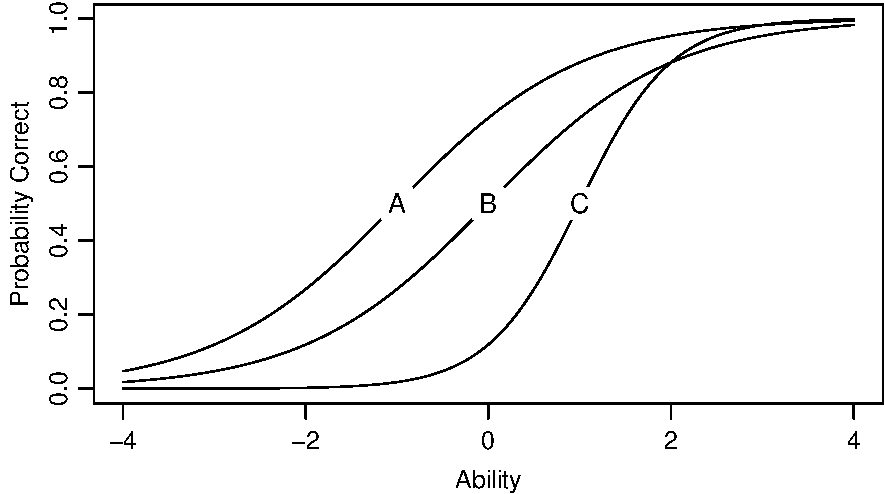
\includegraphics{p_files/figure-latex/f2pl-1.pdf}
\caption{\label{fig:f2pl}Item response curves from Model 2PL. Items have varying location and scale. Items A and B show invariant item ordering, item C violates invariant item ordering when compared to A and B.}
\end{figure}

Ideally, any psychometric model would be \emph{a priori} agnostic as to whether items order. A good measurement model would have the flexibility to account for item orderings and violations of these orderings, depending on the data obtained. Unfortunately, the most popular logistic IRT models are not agnostic. Instead they make \emph{a priori} commitments to item ordering or its violation.

A leading logistic item-response model is the Rasch model (Rasch, 1960). Here, item response curves are specified to be translations of one another. Item A and Item B in Figure~\ref{fig:f2pl} show this translation. The items only differ in average difficulty. Rasch models are certainly endorsed by some psychometricians on philosophical grounds (Wright, 1977). Yet, the vast majority of applications use models more richly parameterized than the Rasch model. The main concern is that the Rasch model's constraint of translated items may be too constraining to provide for an adequate statistical description of the data. For further distinction between philosophical arguments and statistical arguments for and against the Rasch model, see Andrich (2004).

The leading logistic item-response model is called the two-parameter logistic, or 2PL. Two-parameter IRT models, such as 2PL, have an additional parameter, discriminability. In Figure~\ref{fig:f2pl}, Items A and B have the same discriminability parameters; Item C has a different discriminability than Items A and B. One of the main advantages of 2PL is statistical flexibility---items may differ from each other in two distinct ways. In 2PL, items order only if they have the same discriminability. The 2PL model therefore enforces item crossings. If two items have different discriminability parameters, then the response curves must cross. This property may strike some as surprising; after all, if two items are far apart in difficulty, it may appear that they do not cross. Nonetheless, as a matter of mathematical fact, the curves must cross even if the crossing occurs at extreme ability values where the curves are very close to floor or ceiling in value. Whereas the Rasch model forces all items to order, 2PL forces at least some items---those with different discriminabilities---to not order. By choosing between the Rasch model and the 2PL, the analyst makes a content choice that has psychological implications. Either the analyst forces item orderings or forces their violation. And, unfortunately, item ordering is not an open question with the answer reflecting structure in the data.

Most modern psychometric applications are as rich as the 2PL in that items have at a minimum unique difficulty and discriminability parameters with continuous support. And, consequently, in most psychometric applications, it is implicitly stipulated that all items do not order.

\hypertarget{psychophysics-as-an-important-boundary-case}{%
\section{Psychophysics as an Important Boundary Case}\label{psychophysics-as-an-important-boundary-case}}

We find it helpful to consider psychophysics as guidance in designing psychometric models. In psychophysics, we can reasonably assume that stimuli such as light-flashes of varying intensities or tones of varying loudness are one-dimensional. These stimuli serve as items, and, therefore, we can be sure that items are well-ordered.

Morey, Rouder, and Speckman (2008) provides an example. These researchers asked participants to identify digits that were briefly flashed and subsequently masked. The presentation duration of the digits was varied in six levels from 16.7 ms to 100 ms. We treat each of these six levels as an item, and, in this application, we are fortunate to have 90 replicates for each participant-by-item combination. Because there are replicates, it is possible to visualize response proportions without modeling assumptions. Figure~\ref{fig:sl2} shows these proportions for all individuals and items. The pattern is informative. Here, item ordering seems plausible inasmuch as the small violations may be due to sample noise. Moreover, the item-response curves seemingly are not translations of one another, and there is a change of discriminability across the items (Item A discriminates far less between participants than Item F). Hence, we need a model that may account for item orderings while not forcing item-response curves to be shifts of one another.

\begin{figure}
\centering
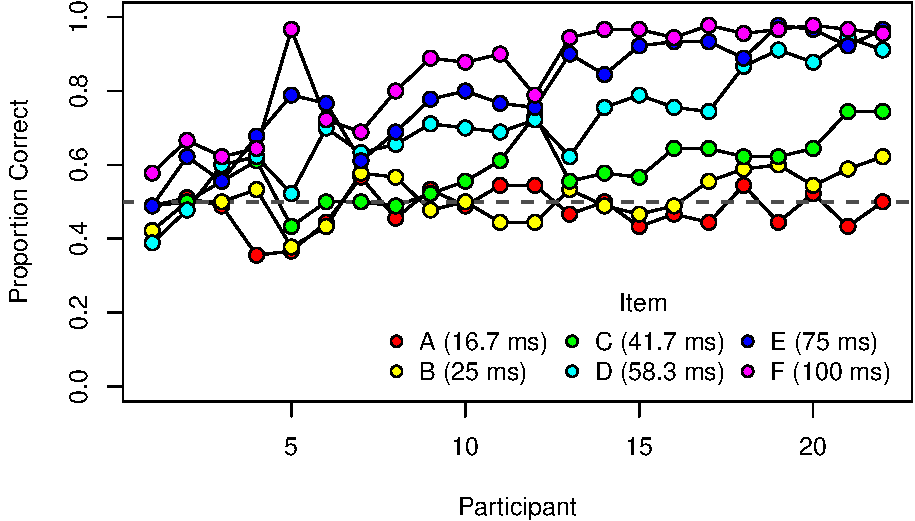
\includegraphics{p_files/figure-latex/sl2-1.pdf}
\caption{\label{fig:sl2}Observed accuracy for all individuals and items in masked digit naming. Items A through F are presentations of 16.7 ms, 25.0ms, 41.7ms, 58.3 ms, 75 ms, and 100 ms. An accuracy value of .5 serves as an at-chance baseline. Data are taken from Morey, Pratte, and Rouder (2018), Figure 7.}
\end{figure}

In addition to the observed proportions, it seems highly plausible from a theoretical perspective that the six items order. It is plausible that all people respond at least as well to digits presented for longer durations than for shorter durations. Indeed, it is hard to conceive of an individual that has better true performance to digits presented say for 16.7 ms than for 41.7 ms. Therefore, we are concerned that no item-response model is appropriate for psychophysical data. While the Rasch model captures item orderings, it does not capture the obvious differences in discriminability among the stimulus durations. It is hard to recommend item-response models in more complicated psychological applications if they miss essential structural properties in areas such as psychophysics where we know much about the items.

In the following, we address this void in psychometrics. We consider IRT models that are as richly parameterized as 2PL but do not force an \emph{a priori} commitment to item orderings or their violations. We view these models as respecting the key psychological property of whether items have the same effect on every individual or different effects on different individuals. The models generally follows cognitive psychometric principles, simply stated as \enquote{models that have more cognitive content than most standard psychometric models, and yet the models are simple enough to allow detailed statistical analysis} (Batchelder, 1998, p. 341).

\hypertarget{shift-scale-links}{%
\section{Shift-Scale Links}\label{shift-scale-links}}

To develop our approach, we first highlight the structural and distributional assumptions in 2PL. The structural property is:\\
\[
p_{ij} = G\left(\frac{\theta_j-\alpha_i}{\beta_i}\right),
\]
where \(p_{ij}\) is the probability of a correct response for the \(j\)th individual on the \(i\)th item, \(i=1,\ldots,I\), \(j=1,\ldots,J\). The parameter \(\theta_j\) is the ability of the \(j\)th individual; the parameters \(\alpha_i\) and \(\beta_i\) are respectively the location and scale of the \(i\)th item. The function \(G\), the link, is monotonically increasing.

In 2PL, the distributional assumption is that \(G\) is the logistic link given by \(G(x)=1/(1-\exp(-x))\). In the model, the parameter \(\alpha_i\) describes the center of the link and parameter \(\beta_i\) describes the scale. This logistic link can be classified as a location-scale link. An example of the 2PL model is shown by the three items in Figure~\ref{fig:f2pl}. The centers are denoted by the letter, and all three items have different centers. Item A and B have the same scale; Item C has a larger scale. A violation of invariant item ordering occurs whenever two items have different scale parameters \(\beta_i\). Importantly, there is no restriction on \(\beta_i\) that allows for item ordering \emph{except} when \(\beta_i\), i.e.~the discriminability, is the same for all items.

\hypertarget{exponential-link}{%
\subsection{Exponential Link}\label{exponential-link}}

The main insight here is that location-scale models with unbounded support, such as 2PL, lead to the critical flaw where scale changes necessarily violate item ordering. One way of avoiding this problem is to change the link. Here, we promote \emph{shift-scale} links. In a shift-scale link, the location parameter serves to shift the bound on support. One possibility is the exponential link, \(G(x)=1-\exp(-x)\) for \(x>0\). With this link the probability of a correct response is
\[
p_{ij} = \left\{\begin{array}{cc}
1-\exp\left(-\frac{\theta_j-\alpha_i}{\beta_i}\right), & \theta_j \geq \alpha_i,\\
0, & \theta_j < \alpha_i.
\end{array}\right.
\]

\begin{figure}
\centering
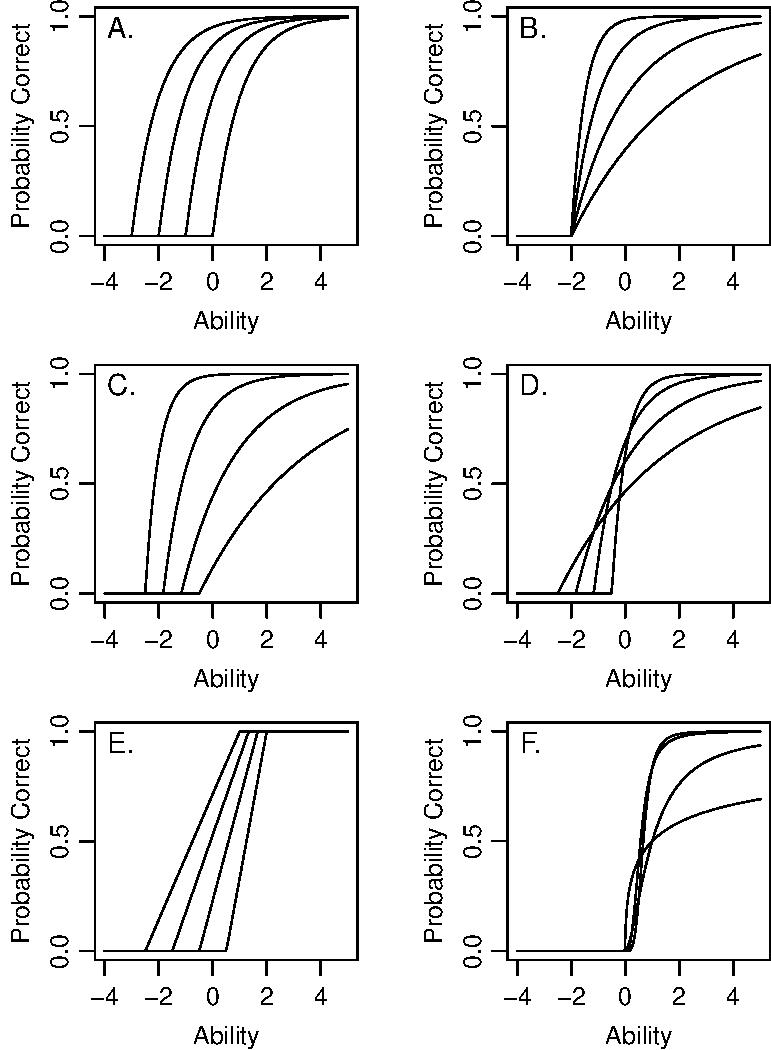
\includegraphics{p_files/figure-latex/f2pe-1.pdf}
\caption{\label{fig:f2pe}Item response curves from shift-scale and unipolar models. A. Changes in shift with constant scale preserve item orderings. B. Changes in scale with constant shift preserve item orderings. This property is not true for 2PL. C. Changes in shift and scale preserve item ordering so long as scale increases with shift. D. When shift increases and scale decreases, item ordering is violated. E. A uniform link provides an account of item ordering without forcing a relationship between shift and scale. F. The conventional unipolar link violates item ordering.}
\end{figure}

The model is analogous in some regards to 2PL and parameters \(\alpha\) and \(\beta\) play the same role as locating and scaling the distribution. The larger the location parameter \(\alpha\), the more difficult the item; The smaller the scale parameter \(\beta\), the higher discriminability between individuals with different ability. Figure~\ref{fig:f2pe} shows a few sets of item response curves from the shifted exponential model. In Panel A, the items differ only in shift, and item response curves are translations of one another. Item ordering is evident, and the model is analogous to the Rasch model, albeit with a different link. In Panel B, the items differ only in scale, and again item ordering is evident. This pattern contrasts with 2PL because in 2PL scale changes necessitate violations of item orderings. Panel C shows items where shift and scale increase for each successive item achieving item ordering as well. Panel D shows how violations of item orderings come about in the model---here, increases in shift correspond to decreases in scale. Figure~\ref{fig:f2pe} shows the desirable flexibility of the 2PE model with respect to item ordering. Item ordering occurs for two items \(i_1\) and \(i_2\) if \(\alpha_{i_1} > \alpha_{i_2} \iff \beta_{i_1} \geq \beta_{i_2}\).

We refer to the parameter \(\alpha\) as a shift parameter. Shift parameters are location parameters that also define the bound of support for a distribution. The key property of the 2PE model is the shift parameter, and in this parameterization, scale increases make items harder for all people.

\hypertarget{uniform-link}{%
\subsection{Uniform Link}\label{uniform-link}}

We also considered the uniform link, which is \(G(x)=x\) of \(x\in[0,1]\). With this link,
\[
p_{ij} = \left\{\begin{array}{cc}
0 & \theta_j<\alpha_i\\
\frac{\theta_j-\alpha_i}{\beta_i}, & \alpha_i \leq \theta_j \leq \alpha_i+\beta_i,\\
1, & \theta_j > \alpha_i+\beta_i .
\end{array}\right.
\]
Here, the parameter \(\alpha\) describes the shift, that is, the lower bound of support, and the parameter \(\beta\) describes the scale, or in this case, the width of the uniform. The upper bound of support is given by \(\alpha+\beta\). Item ordering conditioning again holds for two items if \(\alpha_{i_1} > \alpha_{i_2} \iff \alpha_{i_1} + \beta_{i_1} \geq \alpha_{i_2}+\beta_{i_2}\).

One advantage of the uniform over the exponential is that items need not increase in variance with mean to imply item ordering. With the exponential, item ordering implies that increases in shift are associated with increases in scale. Or, restated, as an item becomes more difficult, it becomes less discriminable.

Discriminability and difficulty are better decoupled with the uniform link. Figure~\ref{fig:f2pe}E shows an example. Here invariant item ordering occurs even though the width decreases with the shift, that is, more difficult items have greater discriminability. Hence, the uniform may be the most flexible two-parameter model---it can describe item orderings and violations of orderings, and item orderings do not force a specific relationship between shift and scale. This advantage will be consequential in application.

\hypertarget{unipolar-links}{%
\subsection{Unipolar Links}\label{unipolar-links}}

The above shift-scale links are alternatives to the more conventional logistic link. There are many such alternatives in psychometrics, though, to our knowledge, most of the parametric alternatives are not designed to address the issue of item ordering. One recent development is the proposal of \emph{unipolar} models where latent abilities are constrained to be positive and where response curves exist on the positive half line (Lucke, 2015; Ramsay, 1989). Because these model exist on bounded support, they too have the potential to account for both item-ordering and violations of it. Yet the conventional unipolar model, say that of Lucke (2015), enforces the violation of item ordering just as 2PL does. The Lucke model is

\[
p_{ij} = \left\{\begin{array}{cc}
0 & \theta_j< 0\\
\frac{\alpha_i\theta_j^{\beta_i}}{1+\alpha_i\theta_j^{\beta_i}}, & \theta_j > 0.
\end{array}\right.
\]

Here, any change in \(\beta_i\), the shape parameter, across two items necessarily forces a violation of an item ordering. Figure~\ref{fig:f2pe}F shows an example of this violation. If one were to assess item ordering in a unipolar setup, a more appropriate link than the Lucke model is the cumulative density function of a two-parameter gamma distribution. The parameters for this distribution are scale and shape. If either parameter is adjusted while holding the other constant, then the resulting item-response curves order. Hence, ordering may be achieved two ways (either in scale or shape), and so long as shape and scale increase together, item ordering is guaranteed. Violations come about when shape decreases with scale.

In the sequel, we develop the shift-scale models discussed above where ability has full support. We retain three models: the two-parameter logistic (2PL), the two-parameter exponential (2PE), and the two-parameter uniform (2PU). The 2PL merely serves as a comparison for readers familiar with current psychometric models. The 2PE and the 2PU are used to assess item ordering, and they are the target of this analysis.

\hypertarget{model-specification-and-analysis}{%
\section{Model Specification and Analysis}\label{model-specification-and-analysis}}

We find it most convenient to analyze IRT models in the Bayesian framework. Needed are priors for the collections of \(\bm \theta\), \(\bm \alpha\), and \(\bm \beta\). We follow the convention of fixing the mean and standard deviation of people's abilities:
\[
\theta_j \stackrel{iid}{\sim} \mbox{Normal}(0,1),
\]
where the normal is parameterized with mean and standard deviation.

The priors for the item parameters are
\[
\begin{aligned}
\alpha_i &\stackrel{iid}{\sim} \mbox{Normal}(c_1,c_2),\\
\beta_i &\stackrel{iid}{\sim} \mbox{Log-Normal}(c_3, c_4),\\
\end{aligned}
\]
where the log-normal is parameterized with mean and standard deviation on the log scale. Constants \((c_1,\ldots,c_4)\) are prior values that need to be set before data analysis. Our goal in choosing \(c_1\) and \(c_2\) is to be weakly informative in comparison to person abilities. For the logistic, we used values of \(c_1=0\) and \(c_2=10\); for the shift parameters in the exponential and uniform, we used values of \(c_1=-1.50\) and \(c_2=10\). We chose \(c_3\) and \(c_4\) by picking values that yielded a reasonable range of item-response curves. Figure \ref{fig:priorCurves} shows this range for the three links and fixed \(\alpha\). For the logistic, \(c_3=-0.20\) and \(c_4=0.50\); for the exponential, \(c_3=0.40\) and \(c_4=0.50\); for the uniform, \(c_3=1\) and \(c_4=0.50\).

\begin{figure}
\centering
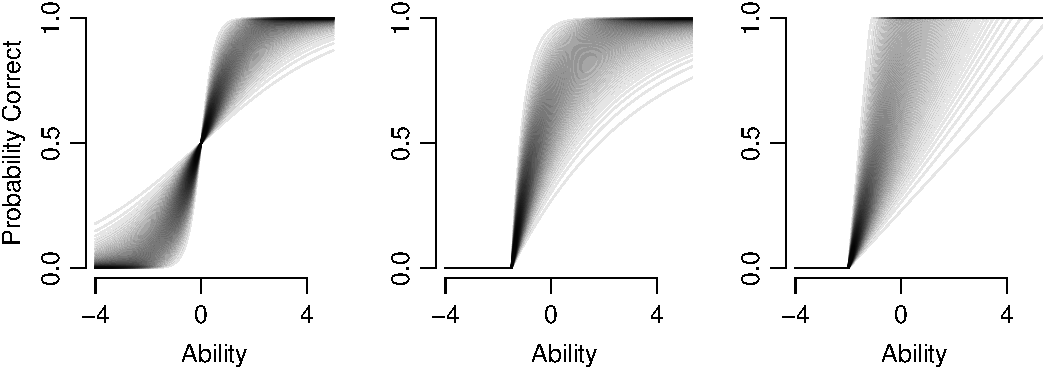
\includegraphics{p_files/figure-latex/priorCurves-1.pdf}
\caption{\label{fig:priorCurves}Range of response curves resulting from the prior on scale (\(\beta\)). There are 99 faint lines, each for a percentile of the lognormal prior. Left: Marginal prior response curves for the logistic model with \(\alpha=0\). Center: Marginal prior response curves for the exponential model with \(\alpha=-2\). Right. Marginal prior response curves for the uniform model with \(\alpha=-2\).}
\end{figure}

We initially derived conditional posteriors for each model and implemented a MCMC chain with Metropolis Hasting sampling of each parameter. Yet, for the shift-scale models, we were unable to achieve good mixing with this approach. The problem is obvious; the shift and scale parameters are too interdependent. A large increase in shift and a corresponding decrease in scale results in likelihoods that change little. Even for models with location-scale links like the 2PL, however, correlation between parameters is an issue. One way of obtaining chains that mix well is to use an alternative sampler that better handles ridges in the likelihood. We developed models based on the \texttt{edstan} package (Furr, 2017) using \texttt{stan} (Stan Development Team, 2018), which employs Hamiltonian sampling (Neal, 2010). The \texttt{R} code is integrated into this manuscript and can be found at \url{https://github.com/PerceptionAndCognitionLab/irt-2pe}.

\hypertarget{applications}{%
\section{Applications}\label{applications}}

To assess whether item ordering holds in common IRT applications, we reanalyzed a few readily-available sets from the \texttt{mirt} (Chalmers, 2012) and \texttt{sirt} (Robitzsch, 2016) packages as well as for the Morey et al. (2008) data previously presented.

\hypertarget{lsat-6}{%
\subsection{LSAT-6}\label{lsat-6}}

The classical LSAT-6 data set, from Thissen (1982), consists of the responses of one-thousand individuals to five dichotomously scored items from the Law School Admissions Test, Section 6. To examine mixing, we ran a single chain for 800 iterations, the first 200 of which served as a burn-in. The quality of mixing was assessed by inspection of chains and by the effective samples statistic. Figure~\ref{fig:LSAT6Chains} shows the trace plots. The rows are for the three models; the columns are for the best (left) and worst (right) mixing item parameters. As can be seen, mixing, while not particularly good, is sufficient. The effective sample sizes (Ripley, 1979) at worst are 1/10 the nominal values, and obtaining hundreds or thousands of samples is not particularly time consuming. Hence, posterior distributions may be estimated to a reasonable degree of confidence.

Figure~\ref{fig:LSAT6}, left column, shows the bivariate posterior samples for all item parameters. There are five clouds, with one cloud for each item in the set. The bivariate posterior mean for each item is located by the letter. The first row is for the 2PL for comparison. Here we see that the LSAT6 data set has a limited resolution. Items A and E are particularly easy (they correspond to accuracies of .92 and .87), and, given this ease, these items yield variable and correlated estimates of difficulty and discriminability across all models. In fact, given the resolution of the data set, if we were measuring ability, we think the Rasch model would be highly appropriate. Importantly, even though posterior estimates of item scales \(\beta\) do not vary by a lot across items, violation of item ordering is necessarily present.

The second and third row show the results for the exponential and uniform links, respectively. If we focus on the exponential link, we see that item ordering may approximately hold. Overall, it seems that Item A has the smallest shift and scale, and the remaining items increase in shift while increasing in scale, with a small violation between items B and C. A similar pattern holds for the uniform link, and item ordering seems even more plausible here. The right column shows corresponding item-response curves evaluated at the posterior means. Here the lack of substantial crossing in the midsection of the curves for all three models bolsters the plausibility of item ordering.

\begin{figure}
\centering
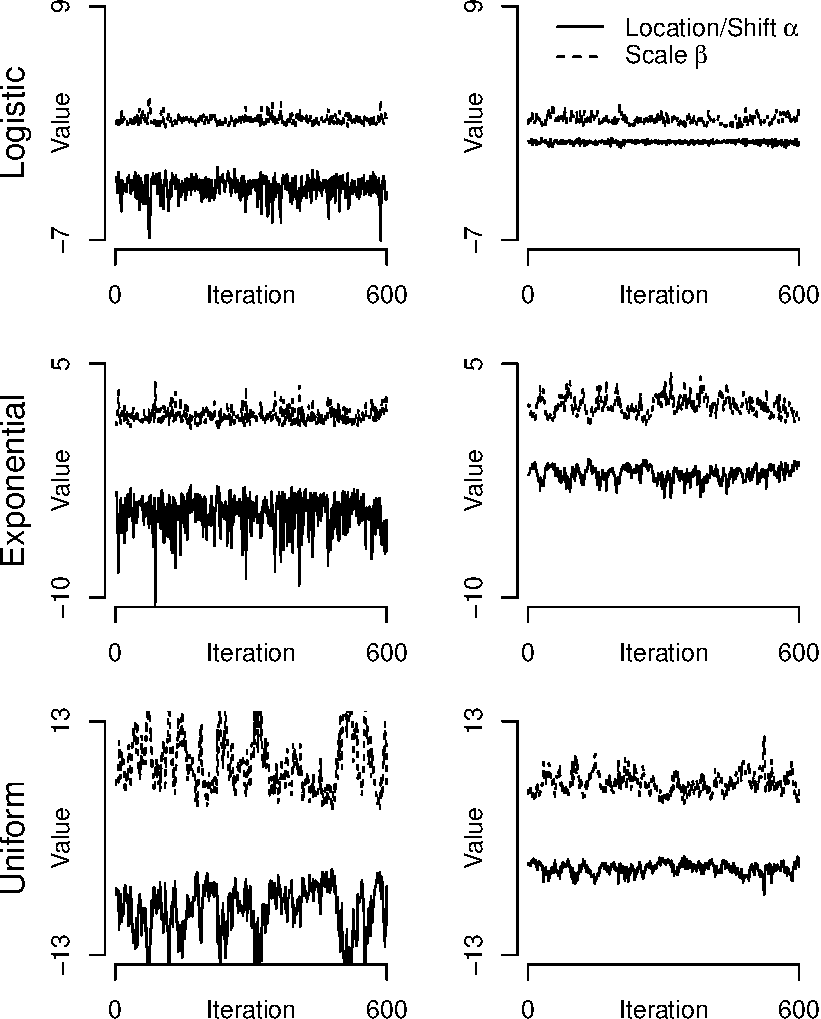
\includegraphics{p_files/figure-latex/LSAT6Chains-1.pdf}
\caption{\label{fig:LSAT6Chains}MCMC trace plots for the items with the most autocorrelation (left) and the least autocorrelated (right) chains.}
\end{figure}

\begin{figure}
\centering
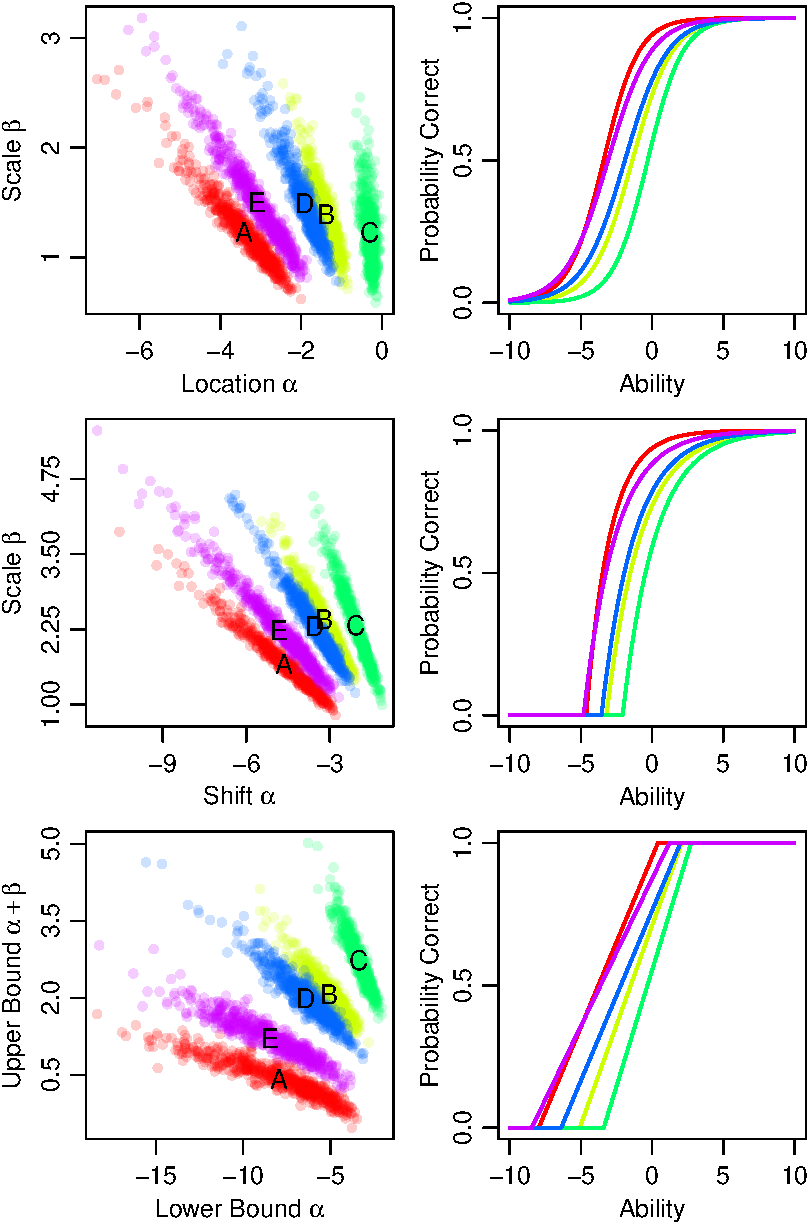
\includegraphics{p_files/figure-latex/LSAT6-1.pdf}
\caption{\label{fig:LSAT6}Results for the LSAT-6 data set. The first column shows the bivariate posterior distributions of item parameters for the five questions. The second column shows the item response curves evaluated at the posterior means. Rows show results for the logistic, exponential, and uniform models, respectively.}
\end{figure}

\hypertarget{lsat-7}{%
\subsection{LSAT-7}\label{lsat-7}}

The LSAT-7 data set, from Bock and Lieberman (1970), consists of the response of one-thousand individuals to five dichotomously scored items from the Law School Admissions Test, Section 7. Figure~\ref{fig:LSAT7}A shows the bivariate posterior samples for all item parameters for the logistic, exponential, and uniform models. There are five clouds, with one for each item in the set. For both the exponential and the uniform link we see a clear violation of item ordering. Consider Items E and C; Item E has a smaller shift but larger scale than Item C. The violation of ordering is also prominent in the right column of Figure~\ref{fig:LSAT7}, which shows the derived item response curves at posterior mean values.

The seeming item ordering for the LSAT-6 and the violation of item ordering for LSAT-7 are easily explained. For the LSAT-6 items, test-takers had to identify a figure that could be classified as belonging to one of two groups of figures, and this skill appears to be relatively homogeneous (Bock \& Lieberman, 1970). For the LSAT-7 items, test-takers had to classify statements as supporting or rejecting a resolution, and the items were quite heterogeneous (Bock \& Lieberman, 1970).

\begin{figure}
\centering
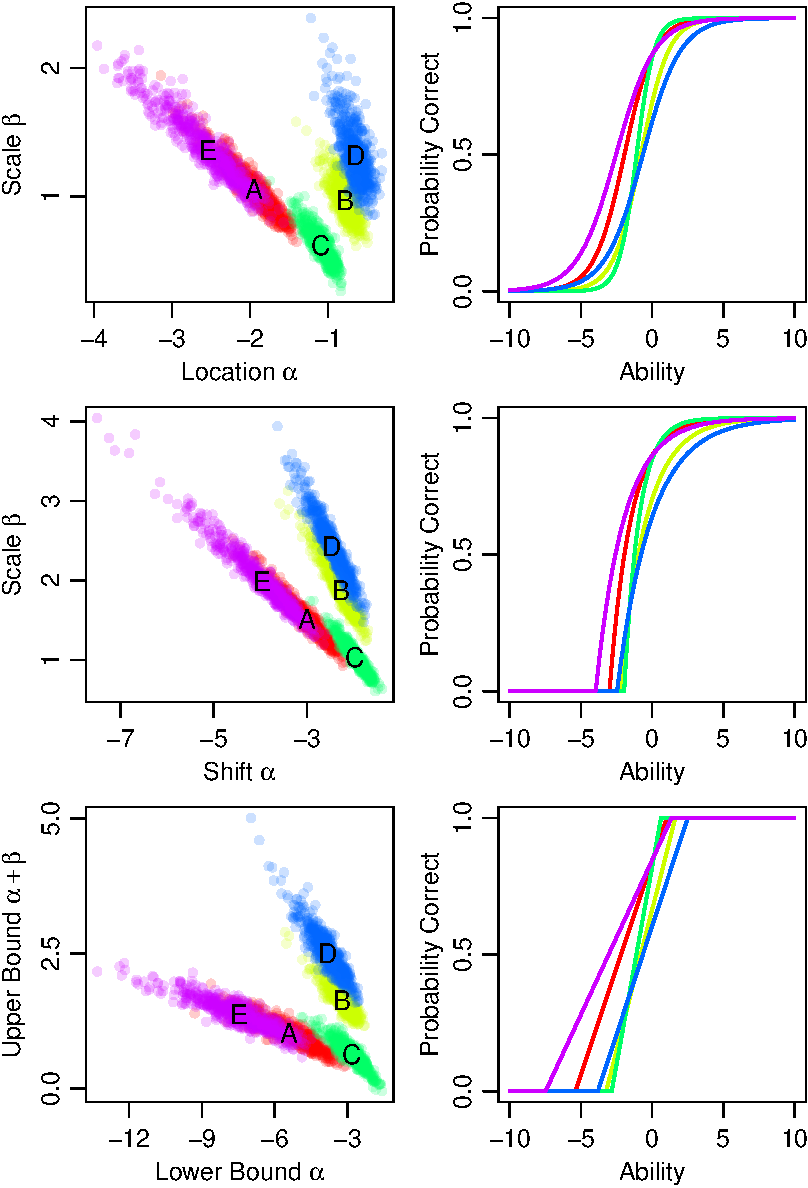
\includegraphics{p_files/figure-latex/LSAT7-1.pdf}
\caption{\label{fig:LSAT7}Results for the LSAT-7 data set. The first column shows the bivariate posterior distributions of item parameters for the five questions. The second column shows the item response curves evaluated at the posterior means. Rows show results for the exponential and uniform models, respectively.}
\end{figure}

\hypertarget{masked-digit-identification}{%
\subsection{Masked Digit Identification}\label{masked-digit-identification}}

One domain in which it is highly plausible that item ordering holds is psychophysics. Previously, we treated stimulus duration as an item variable, and it seems inconceivable that anyone is truly better at identifying stimuli presented at shorter than at longer durations. We reanalyzed the accuracy data in Figure~\ref{fig:sl2} from Morey et al. (2008) with modified 2PE and 2PU models. The modified 2PE model is:
\[
\begin{aligned}
Y_{ij} &\sim \mbox{Binomial}(p_{ij},N_{ij}),\\
p_{ij} &= \frac{1}{2}+\frac{1}{2}\left(1-\exp\left[-\frac{\theta_j-\alpha_i}{\beta_i}\right]\right).
\end{aligned}
\]
The main modification here is a baseline accuracy of .5 rather than zero. In Morey et al.'s experiment, half the digits were less-than-five and half were greater-than-five. Individuals had to choose among these two alternatives. With this experimental setup, individuals unable to identify the stimulus at all have a 50\% chance of correct response. The analogous modification was made for the 2PL and the 2PU models.

The results of the analysis are shown in Figure~\ref{fig:sl2Plot}. Unlike the previous examples, the pattern of parameter estimates (left column) is very much dependent on the model, and the differences are informative. Consider first the exponential model. Here, there is a pronounced nonmonotonicity. The easiest four items, Items C through F, order strongly and are notably different in scale. The hardest two items, Items A (16.7 ms) and B (25 ms), however, order in reverse. The reason for this reverse ordering is more of a statistical issue than any statement about the items. Items A and B correspond to the shortest stimulus durations, and inspection of Figure~\ref{fig:sl2Plot} reveals that it is highly likely that none of the individuals could identify any of the targets above baseline. In this case, there is no information from the performance data other than the shift is quite high. The scale, in particular, reflects only the prior settings, which are lower in value than the data-driven value for Item C. The posterior on scale reflects the prior to a greater and greater degree, that is, for harder items, the scale estimates may actually decrease in value depending on the prior settings. We have confirmed this excessive dependency for hard items by trying various values of priors, and they do have the described effect.

This behavior is not unique to the 2PE. In any two-parameter location-scale IRT model, including 2PL, if all participants perform near baseline on an item, it is very difficult to estimate scale values. This can be seen in the first row for Figure~\ref{fig:sl2Plot}. Posterior samples for item A are extremely spread and mainly reflects the prior.

The pattern for the uniform model, however, is different. Here, the items order! The difference occurs because the uniform model does not require increasing scale with shift for item ordering. Certainly, the estimates of the scale parameter, in this case the width of the uniform, regress to the prior for the hard items. Yet, this regression does not translate into a violation of item orderings. In fact, the width of the uniform for item A is the lowest of all items. Yet, the items still order because the shift is much bigger.

Based on this behavior, we think the uniform link is preferable to the exponential link. Here is a case where requiring decreased discriminability with increased difficulty makes no sense. By using the uniform link rather than the exponential, we can meet the benchmark requirement that physical stimuli order even in the case of extreme levels of performance.

\begin{figure}
\centering
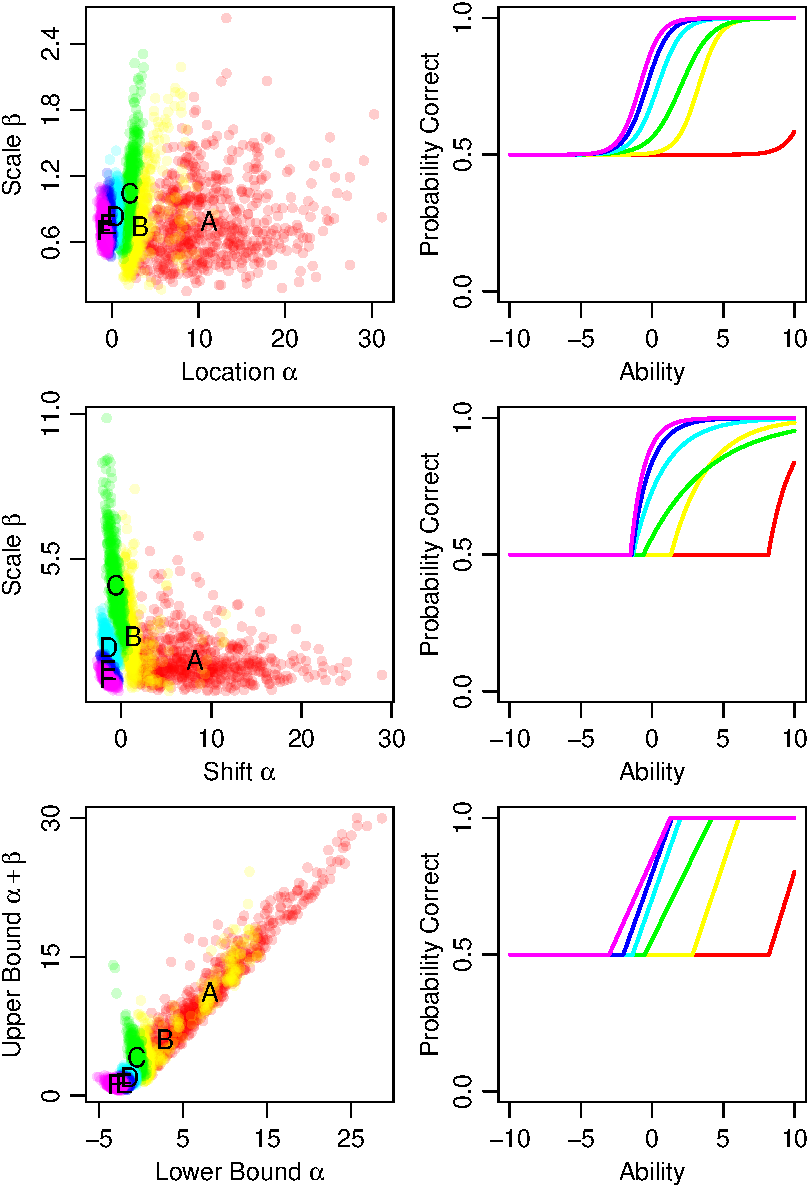
\includegraphics{p_files/figure-latex/sl2Plot-1.pdf}
\caption{\label{fig:sl2Plot}Results for the masked identification data set. The first column shows the bivariate posterior distributions of item parameters for the six durations. The second column shows the item response curves evaluated at the posterior means. Rows show results for the exponential and uniform models, respectively.}
\end{figure}

\hypertarget{bayes-factor-assessment-of-orderings}{%
\section{Bayes Factor Assessment of Orderings}\label{bayes-factor-assessment-of-orderings}}

The two-parameter uniform performs well in the three applications. In particular, it remains agnostic to whether items order or not. Moreover, the model may be used to formally state the strength of evidence from data for invariant item ordering. Here is how:

We follow Klugkist, Laudy, and Hoijtink (2005) in using a counting-based approach to compute the Bayes factor. Before the data are observed, the probability that any \(I\) items will order is \((I!)^{-1}\). Hence, the prior odds that items order is
\[
R_0 = \frac{(I!)^{-1}}{1-(I!)^{-1}}
\]

The posterior probability that the item orders may be computed in the MCMC chain by simply counting how many iterations the ordering of shape estimates matches the ordering of the scale estimates. Let \(\bm \alpha^{[m]}=(\alpha_1^{[m]},\ldots,\alpha_I^{[m]})\) be the I-dimensional vector of shift parameters on the \(m\)th iteration. Likewise, let \(\bm \beta^{[m]}\) be the vector of scale parameters, and let \(\bm \gamma^{[m]}=(\alpha_1^{[m]}+\beta_1^{[m]},\ldots,\alpha_I^{[m])}+\beta_I^{[m]})\) be the vector of the upper bound of the uniform on the \(m\)th iteration. Let \(O(\bm \alpha^{[m]})\) and \(O(\bm \gamma^{[m]})\) be the rank orders of the lower and upper bounds, respectively, and let \(T^{[m]}=1\) if these orders are equal and \(T^{[m]}=0\) otherwise. Then, the posterior probability that the items order is simply the average of \(\bm T\), \(\bar{T} = \sum_m T^{[m]}/M\), where \(M\) is the number of iterations in the chain. The posterior odds is therefore
\[
R_1=\frac{\bar{T}}{1-\bar{T}}.
\]
The Bayes factor is simply the ratio \(R_1/R_0\).

We evaluated the Bayes factor for the three applications. For SAT6 and masked identification, the applications where item ordering seems plausible, the Bayes factors were 10.30-to-1 and 469-to-1, respectively. For the SAT7, where item ordering is obviously violated, we did not sample an iteration where the orders matched. Hence, to get an upper bound on the Bayes factor, we can assume there would be a match on the \(M+1\) iteration, and doing so yields an upper bound of about 0.20-to-1. The odds that the order is violated is at least 5-to-1 and likely much, much greater. Gaining a more accurate estimate is just a matter of increasing the number of iterations.

The above counting approach works well only for a small number of items. It scales exceedingly poorly with increasing number of items as the number of iterations must keep up with the factorial function. Whether there are feasible alternative computational approaches for large item sets is to our knowledge unknown and remains outside the scope of this paper.

\hypertarget{general-discussion}{%
\section{General Discussion}\label{general-discussion}}

Standard IRT models such as the Rasch model and 2PL make strong substantive commitments about item ordering. In the Rasch model all items must order; in 2PL all items must not order. These commitments, in our view, are not generally applicable and must be assessed on a case by case basis. For example, in psychophysics, where items index levels of physical strength, it is reasonable to expect item ordering. Such an ordering would be in violation of 2PL. While most psychometricians do not use stimuli that vary on a single, physical dimension, the point remains that psychometric models \emph{should} apply to this case as an important boundary. Absent from data, it is difficult to justify a commitment to item ordering or to its violation.

We propose a class of IRT links that are flexible with regard to item ordering. These links allow for item ordering or violations of item ordering depending on the data. The links use bounded support, and in particular the uniform, a link with lower and upper bounds performs well in practice. These links are \enquote{you can have your cake and eat it} links in that one retains the flexibility of a two-parameter model without the strong commitment to violations of item ordering.

We ask psychometricians pay heed to a basic, almost minimalist element of psychological content, that is, whether items in a context vary consistently across all people. More pragmatically, we believe domains should be classified as admitting item orderings or violating item orderings. And when they admit a natural ordering, the claim that the items measure a unidimensional latent meaningful psychological construct is much stronger.

\newpage

\hypertarget{references}{%
\section*{References}\label{references}}
\addcontentsline{toc}{section}{References}

\hypertarget{refs}{}
\leavevmode\hypertarget{ref-Andrich:2004}{}%
Andrich, D. (2004). Controversy and the Rasch model: A characteristic of incompatible paradigms? \emph{Medical Care}, \emph{42}, I7--I16.

\leavevmode\hypertarget{ref-Batchelder:1998}{}%
Batchelder, W. H. (1998). Multinomial processing tree models and psychological assessment. \emph{Psychological Assessment}, \emph{10}(4), 331--344. Retrieved from \url{https://doi.org/10.1037/1040-3590.10.4.331}

\leavevmode\hypertarget{ref-Batchelder:2010}{}%
Batchelder, W. H. (2010). Cognitive psychometrics: Using multinomial processing tree models as measurement tools. In S. E. Embretson (Ed.), \emph{Measuring psychological constructs: Advances in model-based approaches.} (pp. 71--93). American Psychological Association. Retrieved from \url{https://doi.org/10.1037/12074-004}

\leavevmode\hypertarget{ref-Batchelder:Riefer:1990}{}%
Batchelder, W. H., \& Riefer, D. M. (1990). Multinomial processing models of source monitoring. \emph{Psychological Review}, \emph{97}, 548--564.

\leavevmode\hypertarget{ref-Bock:Lieberman:1970}{}%
Bock, R. D., \& Lieberman, M. (1970). Fitting a response model for n dichotomously scored items. \emph{Psychometrika}, \emph{35}, 179--197.

\leavevmode\hypertarget{ref-Chalmers:2012}{}%
Chalmers, R. P. (2012). Mirt: A multidimensional item response theory package for the r environment. \emph{Journal of Statistical Software}, 1--29. Retrieved from \url{https://www.jstatsoft.org/article/view/v048i06}

\leavevmode\hypertarget{ref-DeBoeck:Wilson:2004}{}%
De Boeck, P., \& Wilson, M. (2004). \emph{Explanatory item response models: A generalized linear and nonlinear approach}. New York: Springer-Verlag.

\leavevmode\hypertarget{ref-Furr:2017}{}%
Furr, D. C. (2017). \emph{Edstan: Stan models for item response theory}. Retrieved from \url{https://CRAN.R-project.org/package=edstan}

\leavevmode\hypertarget{ref-Klugkist:etal:2005}{}%
Klugkist, I., Laudy, O., \& Hoijtink, H. (2005). Inequality constrained analysis of variance: A bayesian approach. \emph{Psychological Methods}, \emph{10}(4), 477.

\leavevmode\hypertarget{ref-Lucke:2015}{}%
Lucke, J. F. (2015). Unipolar item response models. In S. P. Reise \& D. Revicki (Eds.), \emph{Handbook of item response theory modeling: Applications to typical performance assessment} (pp. 272--284). New York: Routledge.

\leavevmode\hypertarget{ref-Morey:etal:2008a}{}%
Morey, R. D., Rouder, J. N., \& Speckman, P. L. (2008). A statistical model for discriminating between subliminal and near-liminal performance. \emph{Journal of Mathematical Psychology}, \emph{52}, 21--36.

\leavevmode\hypertarget{ref-Neal:2010}{}%
Neal, R. M. (2010). MCMC using Hamiltonian dynamics. In S. Brooks, A. Gelman, G. Jones, \& X.-L. Meng (Eds.), \emph{Handbook of Markov chain Monte Carlo: Methods and applications}. CRC Press.

\leavevmode\hypertarget{ref-Ramsay:1989}{}%
Ramsay, J. O. (1989). A comparison of three simple test theory models. \emph{Psychometrika}, \emph{54}(3), 487--499.

\leavevmode\hypertarget{ref-Rasch:1960}{}%
Rasch, G. (1960). \emph{Probabilistic models for some intelligence and attainment tests}. Copenhagen: Danish Institute for Educational Research.

\leavevmode\hypertarget{ref-Riefer:etal:2002}{}%
Riefer, D. M., Knapp, B. R., Batchelder, W. H., Bamber, D., \& Manifold, V. (2002). Cognitive psychometrics: Assessing storage and retrieval deficits in special populations with multinomial processing tree models. \emph{Psychological Assessment}, \emph{14}, 184--201.

\leavevmode\hypertarget{ref-Ripley:1979}{}%
Ripley, B. D. (1979). Tests ofrandomness' for spatial point patterns. \emph{Journal of the Royal Statistical Society. Series B (Methodological)}, 368--374.

\leavevmode\hypertarget{ref-Robitzsch:2016}{}%
Robitzsch, A. (2016). \emph{Sirt: Supplementary item response theory models}. Retrieved from \url{https://CRAN.R-project.org/package=sirt}

\leavevmode\hypertarget{ref-Sijtsma:Hemker:2000}{}%
Sijtsma, K., \& Hemker, B. T. (2000). A taxonomy of irt models for ordering persons and items using simple sum scores. \emph{Journal of Educational and Behavioral Statistics}, \emph{25}(4), 391--415.

\leavevmode\hypertarget{ref-Sijtsma:Junker:1996}{}%
Sijtsma, K., \& Junker, B. W. (1996). A survey of theory and methods of invariant item ordering. \emph{British Journal of Mathematical and Statistical Psychology}, \emph{49}(1), 79--105. Retrieved from \url{https://doi.org/10.1111/j.2044-8317.1996.tb01076.x}

\leavevmode\hypertarget{ref-rstan:2018}{}%
Stan Development Team. (2018). RStan: The R interface to Stan. Retrieved from \url{http://mc-stan.org/}

\leavevmode\hypertarget{ref-Thissen:1982}{}%
Thissen, D. (1982). Marginal maximum likelihood estimation for the one-parameter logistic model. \emph{Psychometrika}, \emph{47}, 175--186.

\leavevmode\hypertarget{ref-Wright:1977}{}%
Wright, B. D. (1977). Solving measurement problems with the rasch model. \emph{Journal of Educational Measurement}, \emph{14}(2), 97--116.


\end{document}
